\chapter{النمو الجنيني عند الفقاريات}\label{ch:b2:vertebrate-development}

بيضة الضفدع كرة عرضها مليمتران، قاتمة في الأعلى
شاحبة في الأسفل. وفي غضون يوم تكون قد انقسمت إلى آلاف الخلايا؛
وفي غضون يومين تكون صفيحة من تلك الخلايا قد تدحرجت إلى الداخل عبر
ثلم فصنعت معيًا ووضعت قضيبًا على امتداد الظهر؛ وفي غضون ثلاثة، تكون
الصفيحة فوق القضيب قد انطوت أنبوبًا سيصير الدماغ
والنخاع الشوكي. ولم يُضف شيء سوى الماء. فالمعلومة
التي تحوّل خلية واحدة إلى شرغوف سابح كانت في البيضة و
مورثومها، وطريقة انفراطها --- \omterm{def:b2:vertebrate-development:egg}{التفلج}، والتمعّي،
والتعصّب، واستحثاث كل جزء بجيرانه --- هي
نفسها بيّنًا في سمكة وكتكوت وفأر. يتتبع هذا الفصل
جنين فقاري عبر تلك الخطوات ويصف التجارب التي
بيّنت كيف يُقال لكل جزء منه ماذا يصير.

\section{من البيضة إلى الأريمة}

\begin{definition}[البيضة ومحاورها]\label{def:b2:vertebrate-development:egg}
\index{قطب حيواني}\index{قطب نباتي}\index{مح}\index{تفلج}
بيضة الفقاري مستقطبة قبل الإلقاح: أما \emph{القطب الحيواني} فيحمل
النواة ومعظم السيتوبلازم، و\emph{القطب النباتي} يحمل \emph{المح}،
وهو مخزون البروتين والشحم الذي سيعيش عليه الجنين حتى يتغذى.
ومقدار المح يضبط نمط كل ما يتلو: فبيضة قنفذ البحر أو الثدييات
لا مح لها تقريبًا وتتفلج تامًا إلى خلايا متساوية؛ وبيضة الضفدع
فيها مقدار معتدل وتتفلج تامًا لكن غير متساوٍ
(خلايا صغيرة في الأعلى، وخلايا محية كبيرة في الأسفل)؛ وبيضة السمك أو
الطير كلها مح تقريبًا ولا تتفلج إلا في قرص من السيتوبلازم فوقه.
وفي الضفدع، يثبّت موضع دخول النطفة المحور الثاني:
فتدور القشرة ثلاثين درجة بعيدًا عنه، كاشفةً
\emph{هلالًا رماديًا} مقابل نقطة الدخول، وسيصير ذلك الجانب
الظهر. و\emph{التفلج} سلسلة من التقسمات الخيطية السريعة بلا
نمو --- إذ تتنصّف أقيسة الخلايا في كل مرة --- تقودها
رسائل RNA وبروتينات أمومية مخزونة في البيضة، وتبقى مورّثات الجنين
نفسه صامتة حتى \emph{انتقال منتصف \omterm{def:b2:vertebrate-development:blastula}{الأريمة}}، بعد نحو اثني
عشر انقسامًا.
\end{definition}

\begin{omfigure}
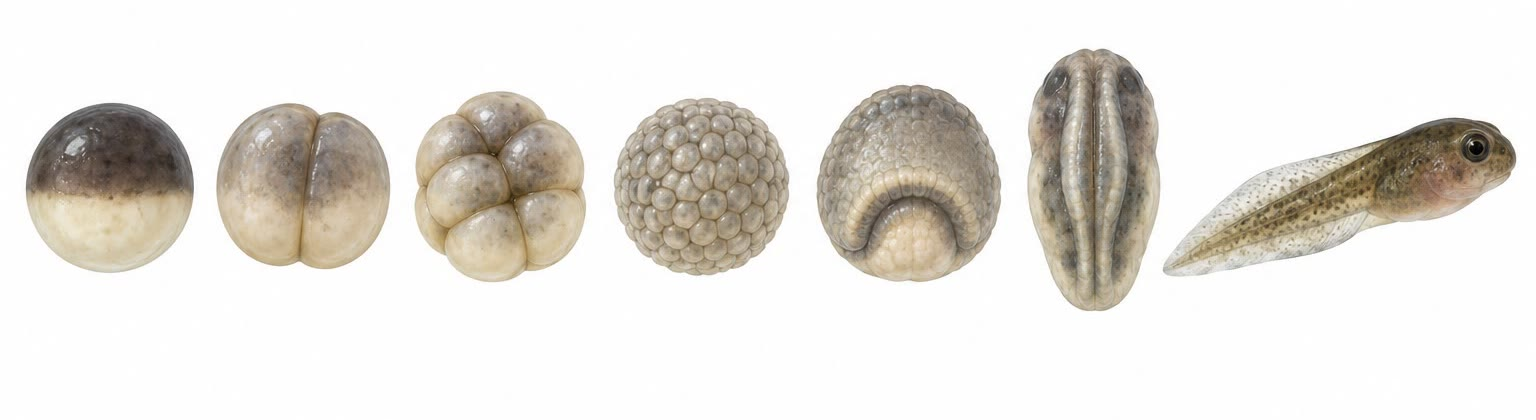
\includegraphics[width=0.9\linewidth]{images/book4/ai/b4-10-frog-development.jpg}

{\small نمو ضفدع من البيضة الملقحة: \omterm{def:b2:vertebrate-development:egg}{تفلج} إلى
\omterm{def:b2:vertebrate-development:blastula}{أريمة}، وتمعٍّ، وعصبولة بطياتها العصبية، ثم
الشرغوف --- وكل ذلك في أيام قليلة، بلا نمو.}
\end{omfigure}

\begin{theorem}[حساب التفلج]\label{thm:b2:vertebrate-development:cleavage}
بعد $k$ تفلجًا متزامنًا تصير بيضة حجمها $V_0$ عددَ $2^{k}$
خلية متوسط حجمها $V_0/2^{k}$ ونصف قطرها $r_0/2^{k/3}$، ويكون
السطح الكلي قد نما بعامل $2^{k/3}$؛ أما نسبة حجم النواة إلى
السيتوبلازم، التي تبدأ قرب $10^{-4}$ في بيضة ضفدع، فترتفع
بعامل $2^{k}$ وتبلغ نسبة خلية عادية ($\sim 0.1$) بعد
نحو عشرة انقسامات. وهذه النسبة المرتفعة --- أي معايرة
مخزون أمومي ثابت من مثبط ما بمقدار متزايد أسّيًا
من DNA --- هي التي تطلق انتقال منتصف \omterm{def:b2:vertebrate-development:blastula}{الأريمة}:
فتبطئ الانقسامات، وتصير غير متزامنة، ويشتعل المورثوم
اللاقحي.
\end{theorem}
\begin{proof}
يُصان الحجم في \omterm{def:b2:vertebrate-development:egg}{التفلج}، فيكون لكل خلية من $2^{k}$ خلية الحجم $V_0
2^{-k}$ ويكون نصف قطرها، بوصفها كرة، $r_0 2^{-k/3}$؛ وتكون مساحتها
الكلية $2^{k}\cdot 4\pi r_0^{2}\, 2^{-2k/3} = 4\pi r_0^{2}\, 2^{k/3}$. وتبقي كل
خلية نواة واحدة ثابتة القياس، فتتقيس النسبة على صورة $2^{k}$
من $10^{-4}$: والقيمة $2^{10} = 1024$ تبلغ بها $0.1$. ويقع انتقال
الضفدع عند الانقسام الثاني عشر، وهو متسق مع
عتبة تُبلغ بعد ذلك بقليل.
\end{proof}
\begin{proof}[شواهد]
أضاف نيوبورت وكيرشنر (1982) DNA زائدًا إلى بيوض الضفدع
فوجدا الانتقال يأتي أبكر بعدد الانقسامات الذي يفيض به DNA؛
ونزع السيتوبلازم كان له الأثر نفسه. فالساعة ليست
زمنًا ولا عدّ انقسامات بل نسبة.
\end{proof}

\begin{definition}[الأريمة]\label{def:b2:vertebrate-development:blastula}
\index{أريمة}\index{جوف الأريمة}
ينتهي \omterm{def:b2:vertebrate-development:egg}{التفلج} إلى \emph{أريمة}: كرة جوفاء (الضفدع، وقنفذ البحر)
أو قرص (السمك، والطير) من بضعة آلاف خلية حول جوف هو
\emph{جوف الأريمة}. وخلاياها لا تزال غير متخصصة في المظهر،
لكنها ليست متكافئة: أما \emph{خريطة المصائر}، المصنوعة بصبغ
رقع من السطح بأصبغة وتتبعها، فتبين أن القلنسوة
الحيوانية ستعطي الجلد والجملة العصبية (\emph{الأديم الظاهر})،
وأن الحزام الاستوائي يعطي العضل والهيكل والكلية والدم
(\emph{الأديم المتوسط})، وأن الكتلة النباتية تعطي المعي وأعضاءه
(\emph{الأديم الباطن}). و\emph{الأوراق الجنينية} الثلاث هذه هي
نفسها في كل فقاري، والخطوة التالية وضعها في مواضعها:
فالأديمان المتوسط والباطن في الخارج ولا بد أن يدخلا.
\end{definition}

\section{التمعّي والتعصّب}

\begin{proposition}[التمعّي]\label{prop:b2:vertebrate-development:gastrulation}
\index{تمعٍّ}\index{ثغرة أريمية}\index{معي بدئي}\index{حبل ظهري}
\emph{التمعّي} هو مجموعة حركات الخلايا التي تحوّل
\omterm{def:b2:vertebrate-development:blastula}{الأريمة} الوحيدة الطبقة إلى \emph{معيولة} ثلاثية الطبقات. وفي
الضفدع يبدأ تحت الهلال الرمادي: فتغير الخلايا هناك شكلها،
قابضةً أطرافها الخارجية حتى تصير كالقوارير، فيتغضن السطح
ثلمًا هو \emph{\omterm{prop:b2:vertebrate-development:gastrulation}{الثغرة الأريمية}}. ومنها ينساب الأديمان المتوسط
والباطن إلى الداخل (\emph{الانقلاب})، متدحرجين فوق الشفة
ومتقدمين على امتداد سقف الجوف؛ وتنتشر القلنسوة الحيوانية
نزولًا لتغطي الخارج (\emph{الانتشار السطحي})؛ وتنغلق \omterm{prop:b2:vertebrate-development:gastrulation}{الثغرة الأريمية}
حلقةً حول آخر الخلايا المحية. وفي الداخل، يكون جوف جديد
مبطن بالأديم الباطن، هو \emph{\omterm{prop:b2:vertebrate-development:gastrulation}{المعي البدئي}}، معيَ المستقبل،
ويكون الأديم المتوسط الذي دخل أولًا، على امتداد الخط الناصف، قد صار
قضيبًا متيبسًا هو \emph{\omterm{prop:b2:vertebrate-development:gastrulation}{الحبل الظهري}}، محور كل جنين فقاري
والبنية التي سمّت الشعبة. وفي الطيور والثدييات تقع
الحركات نفسها عبر شق هو \emph{الخط البدئي}،
في قرص مسطح؛ وفي السمك ينتشر القرص فوق \omterm{def:b2:vertebrate-development:egg}{المح}. و
الرقص يختلف باختلاف \omterm{def:b2:vertebrate-development:egg}{المح}؛ أما النتيجة --- أديم ظاهر في الخارج،
وأديم باطن يبطن المعي، وأديم متوسط بينهما، \omterm{prop:b2:vertebrate-development:gastrulation}{وحبل ظهري} في الخط الناصف
--- فواحدة.
\end{proposition}

\begin{omfigure}
\begin{tikzpicture}[every node/.style={font=\scriptsize}, >=stealth]
  % blastula
  \begin{scope}
    \draw[thick, fill=omDef!15] (0,0) circle (1.3);
    \draw[thick, fill=white] (0,0.2) circle (0.75);
    \fill[omExo!40] (0,0) ++(-1.3,0) arc (180:360:1.3 and 1.3) -- cycle;
    \draw[thick] (0,0) circle (1.3);
    \node at (0,0.2) {جوف الأريمة};
    \node[below, align=center] at (0,-1.45) {أريمة\\قلنسوة حيوانية (بالأزرق)، وخلايا محية (بالرمادي)};
  \end{scope}
  % early gastrula: blastopore forming
  \begin{scope}[xshift=4.2cm]
    \draw[thick, fill=omDef!15] (0,0) circle (1.3);
    \draw[thick, fill=white] (0,0.25) circle (0.7);
    \fill[omExo!40] (0,0) ++(-1.3,0) arc (180:360:1.3 and 1.3) -- cycle;
    \draw[thick] (0,0) circle (1.3);
    \draw[very thick, omThm] (1.0,-0.85) .. controls (0.5,-0.6) and (0.4,-0.3) .. (0.55,0.0);
    \draw[->, thick, omThm] (1.15,-0.7) .. controls (0.6,-0.4) .. (0.4,0.1);
    \draw[omThm] (1.0,-0.85) -- (0.9,-1.25); \node[omThm, anchor=north west] at (0.6,-1.2) {شفة الثغرة};
    \node[below, align=center] at (0,-1.45) {معيولة باكرة\\الخلايا تتدحرج فوق الشفة};
  \end{scope}
  % late gastrula
  \begin{scope}[xshift=8.4cm]
    \draw[thick, fill=omDef!15] (0,0) circle (1.3);
    \draw[thick, fill=omExo!25] (0,0.05) circle (0.95);
    \draw[thick, fill=white] (0.15,-0.1) ellipse (0.55 and 0.4);
    \draw (0.6,-0.3) -- (1.6,-1.15); \node[anchor=west] at (1.6,-1.15) {معي بدئي};
    \draw[very thick, omThm] (-0.9,0.35) .. controls (-0.2,0.6) .. (0.8,0.4);
    \draw[omThm] (0.0,0.48) -- (-0.9,1.55); \node[omThm, anchor=east] at (-0.9,1.55) {حبل ظهري};
    \draw[thick] (1.1,-0.7) -- (1.3,-0.5);
    \node[right] at (1.3,-0.5) {ثغرة أريمية};
    \node[below, align=center] at (0,-1.45) {معيولة متأخرة: ثلاث طبقات،\\وجوف معوي، وحبل ظهري على السقف};
  \end{scope}
\end{tikzpicture}

{\small التمعّي عند الضفدع، في مقطع. تتدحرج الخلايا إلى الداخل
فوق شفة \omterm{prop:b2:vertebrate-development:gastrulation}{الثغرة الأريمية}؛ ويبطن الأديم الباطن جوفًا معويًا جديدًا،
ويصير أول أديم متوسط يدخل هو \omterm{prop:b2:vertebrate-development:gastrulation}{الحبل الظهري} على امتداد الخط الناصف.}
\end{omfigure}

\begin{proposition}[التعصّب والمخطط التنظيمي]\label{prop:b2:vertebrate-development:neurulation}
\index{تعصّب}\index{أنبوب عصبي}\index{قُطَيعة}\index{عرف عصبي}
يثخن الأديم الظاهر فوق \omterm{prop:b2:vertebrate-development:gastrulation}{الحبل الظهري} \emph{صفيحة
عصبية}، ترتفع حافتاها طيتين وتلتقيان في الخط الناصف فتكوّنان
\emph{\omterm{prop:b2:vertebrate-development:neurulation}{الأنبوب العصبي}}، أي الدماغ والنخاع الشوكي المقبلين، ثم يغوص
تحت الجلد؛ وتهاجر خلايا من عرف الطيتين، هي
\emph{\omterm{prop:b2:vertebrate-development:neurulation}{العرف العصبي}}، فتصنع الأعصاب المحيطية،
وخلايا الصباغ، ولب الكظر، ومعظم الوجه. وعلى
جانبي \omterm{prop:b2:vertebrate-development:gastrulation}{الحبل الظهري} يتقطع الأديم المتوسط كتلًا هي
\emph{القُطَيعات}، زوجًا إثر زوج من الرأس إلى الذنب، وهي تعطي
الفقرات وعضلات الجذع والأدمة؛ وينشطر الأديم المتوسط الجانبي
إلى طبقتين تبطنان جوف الجسم وتصنعان القلب
والأطراف؛ ويبرعم أنبوب الأديم الباطن الرئتين والكبد والمعثكلة.
وبنهاية التعصّب يكون للجنين المخطط التنظيمي الفقاري
--- حبل عصبي ظهري فوق \omterm{prop:b2:vertebrate-development:gastrulation}{حبل ظهري}، ومعي بطني، وعضل
متقطع، ورأس --- بطول بضعة مليمترات، وما بقي
من النمو تفصيل الأعضاء من هذا المخطط
(\cref{ch:b2:limb-organogenesis}).
\end{proposition}

\begin{omfigure}
\begin{tikzpicture}[every node/.style={font=\scriptsize}]
  \foreach \x/\lab in {0/{الصفيحة العصبية}, 4.0/{ارتفاع الطيتين العصبيتين}, 8.0/{انغلاق الأنبوب العصبي؛ وهجرة العرف العصبي}} {
    \begin{scope}[xshift=\x cm]
      \draw[thick, fill=omExo!25] (-1.6,0) rectangle (1.6,-1.6);
      \draw[thick, omThm, fill=omThm!30] (0,-0.75) circle (0.28);
      \draw[thick, fill=omProp!30] (-1.3,-0.75) circle (0.32); \draw[thick, fill=omProp!30] (1.3,-0.75) circle (0.32);
      \node[below, align=center, text width=3.4cm] at (0,-1.7) {\lab};
    \end{scope}
  }
  \draw[very thick, omDef] (-1.6,0) -- (-0.7,0) .. controls (-0.3,0.15) and (0.3,0.15) .. (0.7,0) -- (1.6,0);
  \draw[very thick, omDef] (2.4,0) -- (3.3,0) .. controls (3.3,0.9) and (3.6,0.1) .. (4.0,0.0) .. controls (4.4,0.1) and (4.7,0.9) .. (4.7,0) -- (5.6,0);
  \draw[very thick, omDef] (6.4,0.05) -- (9.6,0.05);
  \draw[very thick, omDef, fill=omDef!20] (8.0,-0.3) circle (0.3);
  \foreach \p in {(7.35,-0.4),(8.65,-0.4)} \fill[omDef!70!black] \p circle (0.07);
  \node[omThm, anchor=west] at (9.8,-0.75) {حبل ظهري};
  \node[omProp, anchor=west] at (9.8,-1.15) {قُطَيعة};
  \node[omDef, anchor=west] at (9.8,-0.3) {أنبوب عصبي};
  \node[omDef!70!black, anchor=west] at (9.8,0.1) {خلايا العرف العصبي};
\end{tikzpicture}

{\small التعصّب في مقطع عرضي: يثخن الأديم الظاهر فوق
\omterm{prop:b2:vertebrate-development:gastrulation}{الحبل الظهري} (بالأحمر) وينطوي وينغلق أنبوبًا عصبيًا
(بالأزرق)، بينما يتقطع الأديم المتوسط بجانب \omterm{prop:b2:vertebrate-development:gastrulation}{الحبل الظهري}
قُطَيعات (بالبرتقالي) وتغادر خلايا \omterm{prop:b2:vertebrate-development:neurulation}{العرف العصبي} الطيتين المنغلقتين.}
\end{omfigure}

\begin{omfigure}
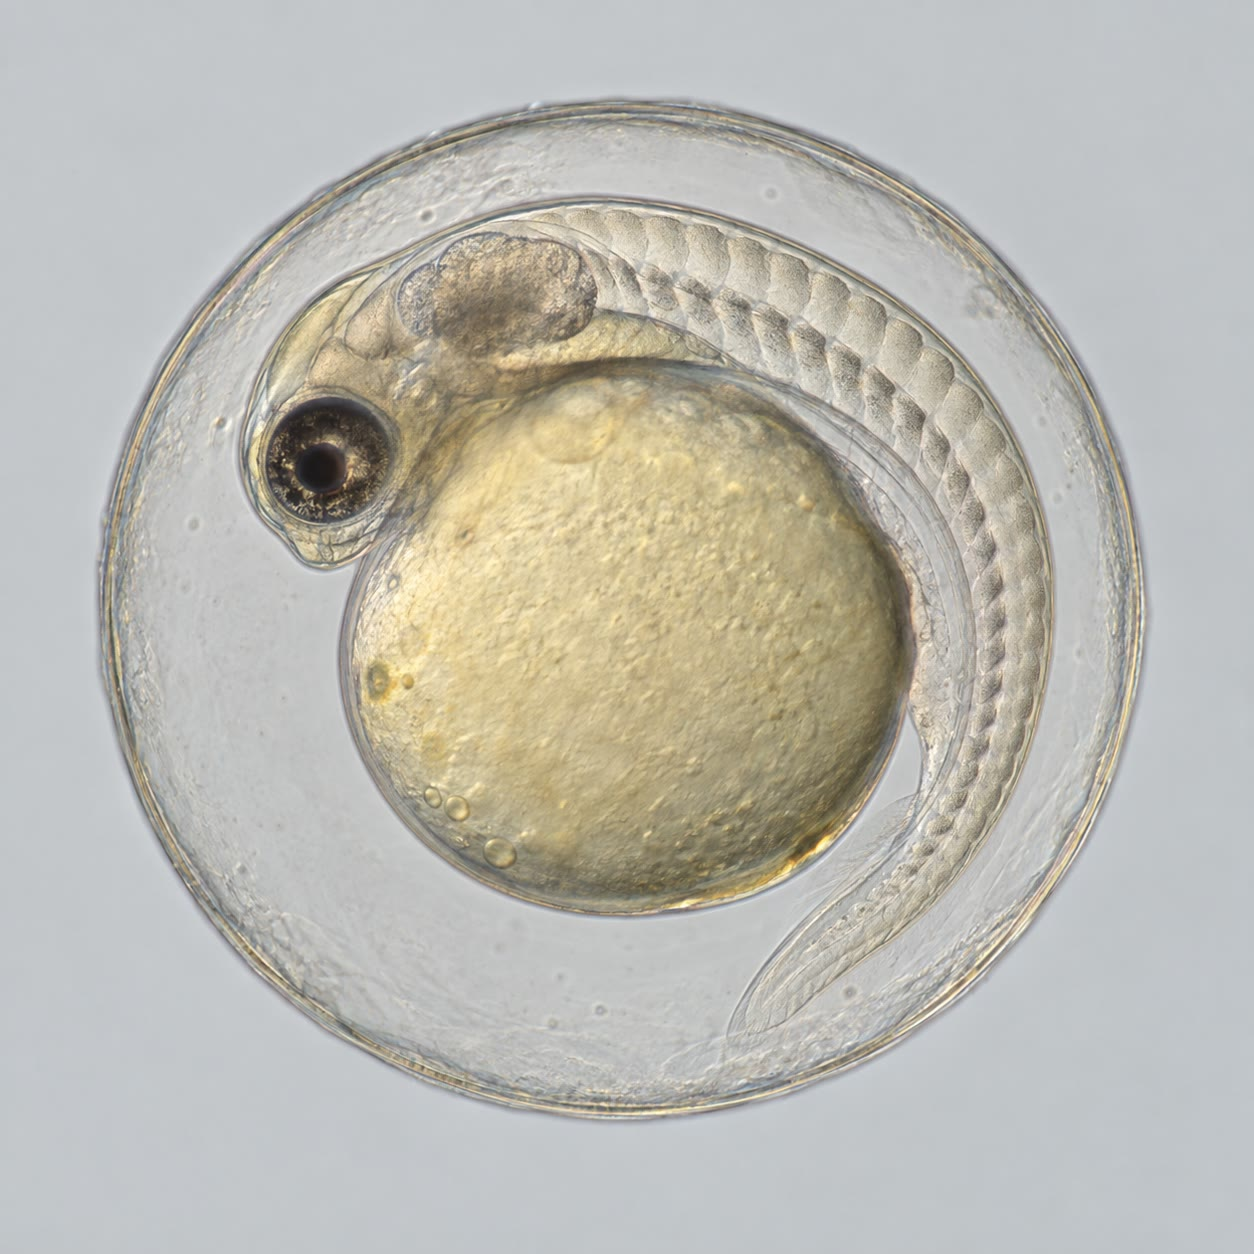
\includegraphics[width=0.42\linewidth]{images/book4/ai/b4-10-zebrafish-embryo.jpg}\hspace{0.04\linewidth}
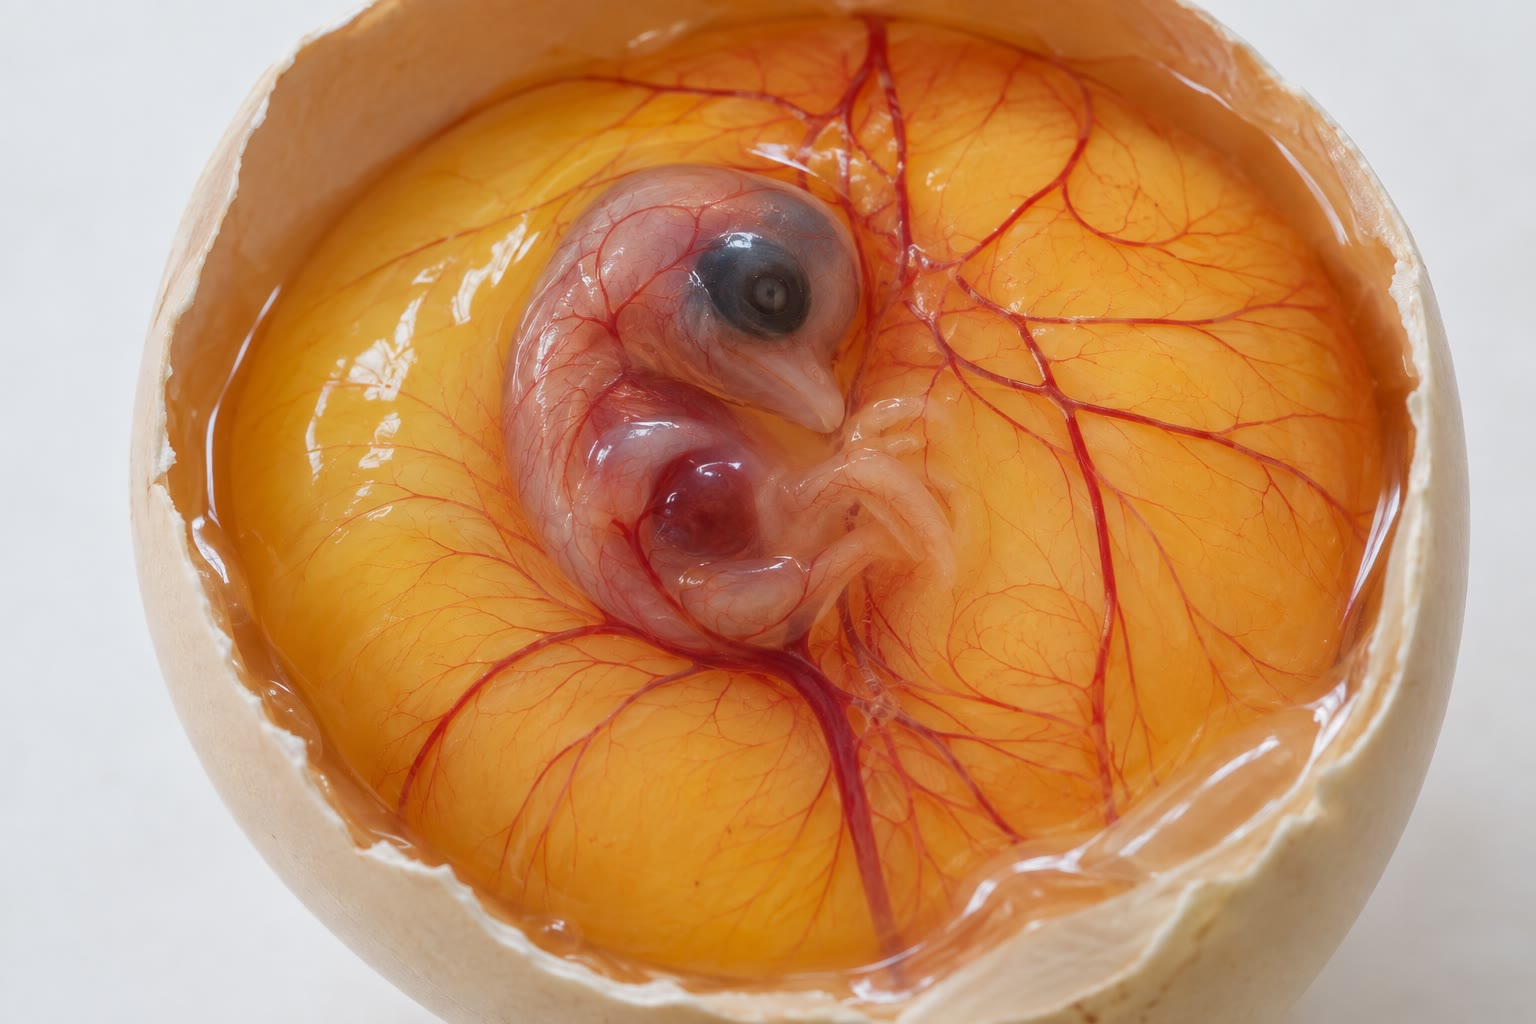
\includegraphics[width=0.5\linewidth]{images/book4/ai/b4-10-chick-embryo.jpg}

{\small على اليمين: جنين سمكة الزرد بعمر يوم داخل مشيمائه،
ملتفًا حول محه، وله عين ودماغ وصف من القُطَيعات.
وعلى اليسار: جنين كتكوت بعمر ثلاثة أيام على محه، وقلبه ينبض
سلفًا وأوعيته تنتشر فوق \omterm{def:b2:vertebrate-development:egg}{المح} لتغذيه.}
\end{omfigure}

\section{الاستحثاث: كيف تعرف الخلايا أين هي}

\begin{definition}[الاستحثاث والأهلية]\label{def:b2:vertebrate-development:induction}
\index{استحثاث جنيني}\index{أهلية}\index{منظّم}
\emph{الاستحثاث} هو الطريقة التي تغير بها مجموعة من الخلايا
مصير مجموعة مجاورة بإشارة؛ ولا بد أن تكون الخلايا المستجيبة
\emph{أهلًا} --- أي قادرة على الجواب، وهي كذلك لمدة
محدودة فقط. والنمو سلسلة من الاستحثاثات: فالخلايا النباتية
تستحث أديمًا متوسطًا في الخلايا فوقها؛ والأديم المتوسط الظهري
--- وهو \emph{المنظّم} عند شفة \omterm{prop:b2:vertebrate-development:gastrulation}{الثغرة الأريمية} --- يستحث
الصفيحة العصبية في الأديم الظاهر فوقه وينمّط الأديم المتوسط على
الجانبين؛ \omterm{prop:b2:vertebrate-development:gastrulation}{والحبل الظهري} يستحث أرض \omterm{prop:b2:vertebrate-development:neurulation}{الأنبوب العصبي}؛ و
الحويصلة البصرية، وهي برعم من الدماغ، تستحث عدسة في الجلد الذي
تلمسه؛ والعدسة تستحث القرنية. وكل نسيج مستحَث يصير
مستحِثًا للذي يليه. والإشارات حفنة من أسر البروتينات
المفرَزة تُستعمل مرارًا --- وهي الأسر نفسها التي تنمّط
طرفًا (\cref{ch:b2:limb-organogenesis}) وتدير، في البالغ،
إشارات \cref{ch:b2:cell-signalling}.
\end{definition}
\begin{proof}[شواهد]
قطع شبيمان ومانغولد (1924) شفة \omterm{prop:b2:vertebrate-development:gastrulation}{الثغرة الأريمية} الظهرية من
معيولة باكرة لنوع من السمندل وطعّماها على الجانب البطني
لنوع آخر، مصبوغ على نحو مختلف بحيث يمكن تمييز خلايا المضيف
والطُّعم. فلم يصر الطُّعم ببساطة ما كان
ليصيره في موضعه: بل تدحرج إلى الداخل، وكوّن حبلًا ظهريًا، و
\emph{استحث الأديم الظاهر البطني للمضيف نفسه} على صنع \omterm{prop:b2:vertebrate-development:neurulation}{أنبوب
عصبي} ثانٍ، وبجانبه قُطَيعات من المضيف --- أي جنينًا ثانيًا
كاملًا، من خلايا المضيف في جله، موصولًا بطنًا ببطن بالأول.
ولم تستطع أي قطعة أخرى من المعيولة ذلك. فسمّيا الشفة
\omterm{def:b2:vertebrate-development:induction}{المنظّم}؛ أما إشاراته (بروتينات تسد العامل المبطّن
BMP) فعُرفت بعد سبعين سنة.
\end{proof}

\begin{omfigure}
\begin{tikzpicture}[every node/.style={font=\scriptsize}, >=stealth]
  % donor
  \draw[thick, fill=omDef!12] (0,0) circle (1.3); \node[above] at (0,1.4) {معيولة واهبة (شاحبة)};
  \draw[very thick, omThm] (0.85,-0.95) arc (-45:-20:1.3); \node[omThm, right] at (1.2,-0.8) {شفة ظهرية};
  \draw[->, thick] (1.6,-0.3) -- (3.4,-0.3);
  % host
  \draw[thick, fill=omExo!45] (5,0) circle (1.3); \node[above] at (5,1.4) {معيولة مضيفة (قاتمة)};
  \draw[very thick, omThm] (5.85,-0.95) arc (-45:-20:1.3); \node[omThm, right] at (6.2,-0.8) {شفتها الخاصة};
  \draw[very thick, omThm] (4.15,0.95) arc (135:160:1.3); \node[omThm, left] at (3.9,1.0) {الطُّعم};
  \draw[->, thick] (6.6,-0.3) -- (8.4,-0.3);
  % result: twinned embryo
  \draw[thick, fill=omExo!45] (10.6,0) ellipse (1.8 and 1.1);
  \draw[very thick, omDef!70!black] (9.2,0.5) .. controls (10.0,0.8) and (11.2,0.8) .. (12.0,0.5);
  \draw[very thick, omDef!70!black] (9.2,-0.5) .. controls (10.0,-0.8) and (11.2,-0.8) .. (12.0,-0.5);
  \node[above] at (10.6,1.2) {النتيجة: محوران};
  \node[anchor=north, align=center, text width=4cm] at (10.6,-1.2) {أنبوب عصبي ثانٍ وقُطَيعات، من خلايا \emph{المضيف}، استحثها الطُّعم};
\end{tikzpicture}

{\small تجربة \omterm{def:b2:vertebrate-development:induction}{المنظّم}. شفة ظهرية مطعّمة على بطن
معيولة أخرى تستحث خلايا المضيف على تكوين محور
جنيني ثانٍ.}
\end{omfigure}

\begin{theorem}[تدرج مورفوجيني]\label{thm:b2:vertebrate-development:gradient}
\index{مورفوجين}
تعمل استحثاثات كثيرة بوساطة \emph{مورفوجين}: أي إشارة يفرزها
منبع، وتنتشر في النسيج، وتقرؤها الخلايا بحسب
تركيزها المحلي --- ففوق عتبة مصير، وفوق عتبة
أعلى مصير آخر. والمورفوجين المنتَج عند منبع مستوٍ بمعدل
$j$ في وحدة المساحة، والمنتشر بمعامل $D$ والمتحلل
بمعدل $k$، له في الحالة المستقرة المنحى الأسّي
\[
c(x) = c_0\,e^{-x/\lambda}, \qquad \lambda = \sqrt{D/k}, \qquad c_0 = \frac{j}{\sqrt{Dk}},
\]
فتكون المسافة التي يهبط عندها التركيز دون
عتبة $T$ هي $x_T = \lambda\ln(c_0/T)$: أي إن نسيجًا يمكن
تنميطه إلى نطق ثابتة العرض بعتبات ثابتة. فمع $D =
\qty{1e-12}{m^2/s}$ (بروتين يبطئه ارتباطه وهو يتحرك عبر
النسيج) و$k = \qty{1e-3}{s^{-1}}$ (وعمر نصف نحو اثنتي عشرة
دقيقة)، يكون $\lambda = \sqrt{10^{-9}}\,\unit{m} \approx
\qty{32}{\micro m}$: أي بضعة أقطار خلوية،
وهو المقياس الذي تُنمَّط عليه الحقول الجنينية. ومضاعفة
المنبع تضاعف $c_0$ وتزيح كل حد إلى الخارج بمقدار $\lambda
\ln 2$.
\end{theorem}
\begin{proof}
في الحالة المستقرة يوازن الانتشار التحلل: $D\,c'' = k\,c$،
وحلها المتناقص هو $c = c_0 e^{-x/\lambda}$ مع $\lambda^2 =
D/k$. والتدفق المغادر للمنبع هو $-Dc'(0) = Dc_0/\lambda = j$،
وهذا يعطي $c_0 = j\lambda/D = j/\sqrt{Dk}$. ووضع $c(x_T) = T$
يعطي $x_T$؛ وتغيير $c_0$ إلى $2c_0$ يضيف إليه $\lambda\ln 2$.
\end{proof}

\begin{omfigure}
\begin{tikzpicture}
\begin{axis}[
  width=0.78\linewidth, height=5.6cm,
  axis x line=bottom, axis y line=left,
  xmin=0, xmax=120, ymin=0, ymax=1.1,
  xlabel={المسافة عن المنبع (\unit{\micro m})}, ylabel={المورفوجين (نسبيًا)},
  xlabel style={font=\small, at={(axis description cs:0.5,-0.13)}, anchor=north},
  ylabel style={font=\small},
  tick label style={font=\small}, xtick={0,32,64,96}, ytick={0,0.5,1},
  clip=false,
]
\fill[omThm!18] (axis cs:0,0) rectangle (axis cs:22,1.05); \node[font=\scriptsize, anchor=south] at (axis cs:11,1.05) {المصير أ};
\fill[omProp!18] (axis cs:22,0) rectangle (axis cs:61,1.05); \node[font=\scriptsize, anchor=south] at (axis cs:41,1.05) {المصير ب};
\fill[omExo!18] (axis cs:61,0) rectangle (axis cs:120,1.05); \node[font=\scriptsize, anchor=south] at (axis cs:90,1.05) {المصير ج};
\addplot[very thick, omDef, domain=0:120, samples=80] {exp(-x/32)};
\draw[dashed, gray] (axis cs:0,0.5) -- (axis cs:22,0.5) -- (axis cs:22,0);
\draw[dashed, gray] (axis cs:0,0.15) -- (axis cs:61,0.15) -- (axis cs:61,0);
\node[font=\scriptsize, anchor=west] at (axis cs:62,0.55) {العتبة 1};
\node[font=\scriptsize, anchor=west] at (axis cs:62,0.2) {العتبة 2};
\end{axis}
\end{tikzpicture}

{\small تدرج مورفوجيني مع $\lambda = \qty{32}{\micro m}$.
تقطع عتبتان النسيج إلى ثلاثة نطق من مصائر الخلايا
تضبط عروضَها $\lambda$ ونسبُ العتبات إلى
تركيز المنبع.}
\end{omfigure}

\begin{example}[قراءة التدرج]\label{ex:b2:vertebrate-development:reading}
في معيولة الضفدع، تصير خلايا المنطقة الهامشية المعرَّضة لمقادير
متدرجة من إشارة من أسرة الأكتيفين، من الجرعة العالية إلى
المنخفضة، حبلًا ظهريًا وعضلًا وكلية ودمًا؛ والخلايا المفرَّقة من
القلنسوة الحيوانية الموضوعة في طبق مع جرعة عتبية تبدّل مصائرها ضمن
عامل اثنين من التركيز. وفي \omterm{prop:b2:vertebrate-development:neurulation}{الأنبوب العصبي}، تنتشر إشارة من
\omterm{prop:b2:vertebrate-development:gastrulation}{الحبل الظهري} وصفيحة الأرض صاعدةً وتحدد، من
الأسفل، العصبونات المحركة ثم أصنافًا متعاقبة من
العصبونات البينية عند عتبات تفصلها بضعة أقطار خلوية. فإحداثيات
الكائن مكتوبة بالتراكيز.
\end{example}

\section{المصير والالتزام وتوقيت القرارات}

\begin{proposition}[متى يثبت مصير خلية]\label{prop:b2:vertebrate-development:commitment}
\index{تحدد}\index{تنظيم جنيني}
\emph{مصير} الخلية ما ستصيره عادةً؛ و\emph{قدرتها}
ما تستطيع أن تصيره إن نُقلت؛ وتكون
\emph{متحددة} حين لا يعود مصيرها يتغير بتغير
محيطها. والأجنة الباكرة \emph{تنظّم}: فكل من أولى فلجتي
الضفدع، إذا فُصلت، تصنع شرغوفًا صغيرًا كاملًا، وأولى
خلايا جنين ثديي \omterm{prop:b2:asexual-reproduction:tissueculture}{كلية القدرة} كلها --- وهكذا تنشأ
التوائم المتطابقة. والتحدد يأتي تدريجيًا وفي
أوقات مختلفة لأنسجة مختلفة: فقطعة من أديم ظاهر لمعيولة
باكرة مطعّمة على البطن تصير جلد بطن، والقطعة نفسها
المأخوذة من معيولة متأخرة تصنع صفيحة عصبية حيثما وُضعت؛
وعند طور برعم الذنب يصنع حقل طرف منقول إلى الخاصرة
طرفًا هناك. أما في معظم اللافقاريات فيثبت المصير باكرًا
بالسيتوبلازم الذي ترثه كل خلية (النمو \emph{الفسيفسائي})
والفلجة المفصولة لا تصنع إلا جزءها. واستراتيجية الفقاريات
--- إبقاء الخلايا مرنة وإخبارها بما تفعل بالاستحثاث ---
هي التي تجعل التوأمة والتجدد وتجربة \omterm{def:b2:vertebrate-development:induction}{المنظّم}
ممكنة.
\end{proposition}
\begin{proof}[شواهد]
ربط شبيمان (1901) أنشوطة شعر حول بيضة سمندل في طور
الخليتين: فإذا وقعت الأنشوطة في مستوي الهلال الرمادي، بحيث
تلقى كل نصف جزءًا منه، تكوّن جنينان كاملان؛ وإذا
وقعت عمودية، بحيث كان لنصف واحد الهلال كله، صنع ذلك
النصف جنينًا وصنع الآخر كرة من نسيج بطني. فالهلال
--- أي \omterm{def:b2:vertebrate-development:induction}{المنظّم} المقبل --- كان الجزء الوحيد الذي لم يكن
ممكنًا تقسيمه.
\end{proof}

\begin{example}[الجدول الزمني لضفدع]\label{ex:b2:vertebrate-development:timetable}
عند \qty{18}{\celsius}: الإلقاح؛ \omterm{def:b2:vertebrate-development:egg}{والتفلج} الأول عند \qty{1.5}{h}،
ثم كل نصف ساعة؛ \omterm{def:b2:vertebrate-development:blastula}{وأريمة} من \num{4000} خلية عند \qty{7}{h}؛
وانتقال منتصف \omterm{def:b2:vertebrate-development:blastula}{الأريمة} عند \qty{8}{h}؛ والتمعّي من \qty{10}{h} إلى
\qty{20}{h}؛ وانغلاق الطيتين العصبيتين عند \qty{30}{h}؛ ونبض القلب عند
\qty{2.5}{d}؛ والفقس والتغذي عند \qty{4}{d}، شرغوفًا طوله
\qty{6}{mm}. وسمكة الزرد تفعل الشيء نفسه في يوم، والكتكوت في ثلاثة،
والفأر في تسعة؛ أما الجنين البشري فيتمعّى في الأسبوع الثالث و
يغلق أنبوبه العصبي بحلول الرابع --- قبل أن تعرف معظم النساء أنهن
حوامل، ولذلك يُوصف الفولات، اللازم لانغلاق \omterm{prop:b2:vertebrate-development:neurulation}{الأنبوب العصبي}،
قبل الحمل.
\end{example}

\section{تمارين}

\begin{exercise}[$\star$]\label{exo:b2:vertebrate-development:1}
عرّف \omterm{def:b2:vertebrate-development:egg}{التفلج} \omterm{def:b2:vertebrate-development:blastula}{والأريمة} والتمعّي والتعصّب، وسمِّ
البنية التي ينتجها كل طور.
\end{exercise}

\begin{exercise}[$\star$]\label{exo:b2:vertebrate-development:2}
أعط الأوراق الجنينية الثلاث، وأربعة أنسجة بالغة تشتق من كل
منها.
\end{exercise}

\begin{exercise}[$\star$]\label{exo:b2:vertebrate-development:3}
كيف يغير مقدار \omterm{def:b2:vertebrate-development:egg}{المح} نمط \omterm{def:b2:vertebrate-development:egg}{التفلج} ونمط
التمعّي؟ قارن ضفدعًا بكتكوت.
\end{exercise}

\begin{exercise}[$\star$]\label{exo:b2:vertebrate-development:4}
ما الاستحثاث؟ أعط ثلاثة استحثاثات بالترتيب الذي تقع به في
جنين ضفدع، مسمّيًا المستحِث والنسيج المستجيب.
\end{exercise}

\begin{exercise}[$\star\star$]\label{exo:b2:vertebrate-development:5}
بيضة ضفدع نصف قطرها \qty{1}{mm} تتفلج اثنتي عشرة مرة. احسب
عدد الخلايا، ومتوسط نصف قطرها، والعامل الذي نما به
سطح الخلايا الكلي. ولماذا يحتاج الجنين إلى السطح الزائد؟
\end{exercise}

\begin{exercise}[$\star\star$]\label{exo:b2:vertebrate-development:6}
تبدأ نسبة النواة إلى السيتوبلازم عند $10^{-4}$ ويقع
انتقال منتصف \omterm{def:b2:vertebrate-development:blastula}{الأريمة} حين تبلغ $0.4$. فبعد كم
انقسامًا؟ وإذا حُقنت البيضة بثلاثة أمثال ما فيها
من DNA، ففي أي انقسام يأتي الانتقال؟
\end{exercise}

\begin{exercise}[$\star\star$]\label{exo:b2:vertebrate-development:7}
مورفوجين له $D = \qty{2e-12}{m^2/s}$ وعمر نصف
\qty{10}{min}. احسب $k$ و$\lambda$. وعتبتاه عند
\qty{50}{\%} و\qty{10}{\%} من تركيز المنبع: أعط
عروض نطق المصائر الثلاثة.
\end{exercise}

\begin{exercise}[$\star\star$]\label{exo:b2:vertebrate-development:8}
في تدرج التمرين السابق يتضاعف المنبع بفعل
\omterm{def:b2:genome-diversification:mutation}{طفرة}. فبكم يتحرك كل حد؟ وماذا لو تضاعف
معدل التحلل بدل ذلك؟
\end{exercise}

\begin{exercise}[$\star\star$]\label{exo:b2:vertebrate-development:9}
صف تجربة شبيمان--مانغولد، وقل لماذا كان لا بد أن يختلف
النوعان في التصبغ، واذكر ما استبعدته النتيجة.
\end{exercise}

\begin{exercise}[$\star\star\star$]\label{exo:b2:vertebrate-development:10}
تنبّأ بنتيجة: (أ) قطعة من صفيحة عصبية مرتقبة لمعيولة
باكرة مطعّمة على البطن؛ (ب) القطعة نفسها من معيولة
متأخرة؛ (ج) قطعة من أديم ظاهر بطني موضوعة فوق \omterm{prop:b2:vertebrate-development:gastrulation}{حبل ظهري} في
معيولة متأخرة؛ (د) \omterm{def:b2:vertebrate-development:induction}{المنظّم} كله منزوعًا من معيولة
باكرة. اشرح كلًا منها بمفهومي \omterm{def:b2:vertebrate-development:induction}{الأهلية} و
التحدد.
\end{exercise}

\begin{exercise}[$\star\star\star$]\label{exo:b2:vertebrate-development:11}
يستغرق \omterm{def:b2:vertebrate-development:egg}{تفلج} الضفدع الأول \qty{90}{min} ويستغرق الأحد عشر التالية
\qty{30}{min} لكل منها، عند \qty{18}{\celsius}؛ وعند \qty{10}{\celsius} تكون كل
خطوة أبطأ بمقدار 2.5 مرة. ففي أي زمن يُبلغ انتقال منتصف
\omterm{def:b2:vertebrate-development:blastula}{الأريمة} عند كل درجة حرارة؟ واشرح لماذا يأتي الانتقال
عند عدد الخلايا نفسه عند الحرارتين، وماذا يقول ذلك
عن الساعة.
\end{exercise}

\begin{exercise}[$\star\star\star$]\label{exo:b2:vertebrate-development:12}
«جنين الفقاري يُبنى بالمحادثة، وجنين اللافقاري
بالوراثة.» ناقش التقابل بين النمو التنظيمي والفسيفسائي،
وعواقبه على التوأمة والتجدد، و
لماذا هو فرق في الدرجة.
\end{exercise}

\section{مسألة: جنين ضفدع موقوت ومنمَّط}

\begin{problem}[{مسألة نهاية الأسبوع --- متابعة جنين ضفدع عبر
التفلج وانتقال منتصف الأريمة والتمعّي والاستحثاث،
مع حساب التدرج المورفوجيني والتنبؤ بالطُّعوم الكلاسيكية،
وتنتهي إلى عدد الخلايا وزمن الانتقال وعروض
نطق المصائر}]
\label{pb:b2:vertebrate-development:1}
بيضة ضفدع نصف قطرها \qty{0.7}{mm} ونواتها نصف قطرها
\qty{0.03}{mm} ومحتواها من DNA هو $c$؛ ويستغرق كل \omterm{def:b2:vertebrate-development:egg}{تفلج}
\qty{30}{min} بعد \omterm{def:b2:vertebrate-development:egg}{تفلج} أول يستغرق \qty{75}{min}. ويقع انتقال منتصف
\omterm{def:b2:vertebrate-development:blastula}{الأريمة} حين يبلغ DNA الكلي $4000\,c$. والمورفوجين: $D =
\qty{1e-12}{m^2/s}$، وعمر نصف \qty{20}{min}، وتركيز منبع
$c_0$، وعتبتان عند $0.4\,c_0$ و$0.08\,c_0$.

\medskip
\noindent\textbf{الجزء الأول --- \omterm{def:b2:vertebrate-development:egg}{التفلج}.}
\begin{enumerate}
  \item احسب حجم البيضة وحجم نواتها، والنسبة الابتدائية
        للنواة إلى السيتوبلازم.
  \item بعد كم تفلجًا يبلغ DNA المقدار $4000\,c$؟ وكم
        خلية؟
  \item وفي أي زمن بعد الإلقاح؟
  \item ما متوسط نصف قطر الخلية عندئذ، وما نسبة حجم النواة
        إلى حجم الخلية إذا حافظت النوى على قياسها؟ علّق.
  \item بأي عامل نما سطح الخلايا الكلي؟
  \item كل \omterm{def:b2:vertebrate-development:egg}{تفلج} يحتاج إلى نسخ المورثوم: فكم DNA اصطُنع
        في المجموع، بوحدات $c$، ولماذا لا يحتاج الجنين
        إلى استنساخ مورّثاته ليفعل ذلك؟
  \item ما الذي يتغير عند الانتقال، وأي تجربة تبين
        أنه يُطلق بنسبة لا بعدّ؟
\end{enumerate}

\medskip
\noindent\textbf{الجزء الثاني --- التمعّي.}
\begin{enumerate}[resume]
  \item أين تتكون \omterm{prop:b2:vertebrate-development:gastrulation}{الثغرة الأريمية} بالنسبة إلى نقطة دخول
        النطفة، وما الذي ثبّت ذلك الموضع؟
  \item اذكر، بالترتيب، الأنسجة التي تتدحرج إلى الداخل عبر
        \omterm{prop:b2:vertebrate-development:gastrulation}{الثغرة الأريمية} ومواضعها بعد ذلك.
  \item يستغرق التمعّي \qty{10}{h} وتقطع الصفيحة المنقلبة
        \qty{2}{mm}. احسب متوسط سرعة الخلية
        بالميكرومترات في الدقيقة وقارنه بأرومة ليفية زاحفة
        (\qty{1}{\micro m/min}).
  \item لماذا يستحيل التمعّي قبل انتقال منتصف
        \omterm{def:b2:vertebrate-development:blastula}{الأريمة}؟
  \item اشرح في جملة واحدة لماذا يكون \omterm{prop:b2:vertebrate-development:gastrulation}{الحبل الظهري}، لا
        \omterm{prop:b2:vertebrate-development:neurulation}{الأنبوب العصبي}، البنية المميزة للحبليات.
  \item يُطبَّق دواء يسد تغير شكل الخلايا عند بداية
        التمعّي. تنبّأ بالجنين.
\end{enumerate}

\medskip
\noindent\textbf{الجزء الثالث --- التدرج.}
\begin{enumerate}[resume]
  \item احسب $k$ من عمر النصف، واحسب $\lambda$.
  \item احسب موضعي العتبتين.
  \item أعط عروض نطق المصائر الثلاثة بالميكرومترات وبعدد
        خلايا قياسها \qty{15}{\micro m}.
  \item يُنصّف المنبع. أعد حساب الموضعين واذكر
        أي نطاق ينكمش أكثر.
  \item خلية على بعد \qty{60}{\micro m} من المنبع تُنقل إلى
        \qty{10}{\micro m} قبل أن يُقرأ التدرج؛ ثم بعده.
        فماذا تصير في كل حالة، ولماذا؟
  \item اشرح لماذا يعطي المنحى الأسّي حدودًا تتوقف
        مواضعها على لوغاريتم قوة المنبع،
        ولماذا يجعل هذا التنميط متينًا.
\end{enumerate}

\medskip
\noindent\textbf{الجزء الرابع --- الطُّعوم.}
\begin{enumerate}[resume]
  \item تنبّأ بنتيجة تطعيم شفة ظهرية على الجانب البطني
        لمعيولة باكرة، وبنتيجة تطعيم منطقة هامشية بطنية
        على الجانب الظهري.
  \item تنبّأ بنتيجة تطعيم شفة ظهرية على الجانب البطني
        \emph{لعصبولة}، واشرح الفرق.
  \item جنين ضفدع في طور الخليتين يُشق على امتداد مستوي
        الهلال الرمادي؛ وآخر عموديًا عليه. تنبّأ
        بالاثنين.
  \item تُقطع قلنسوة حيوانية من \omterm{def:b2:vertebrate-development:blastula}{أريمة} وتُزرع وحدها؛ ثم
        تُزرع القلنسوة نفسها بجانب خلايا نباتية. تنبّأ
        بالأنسجة المتكونة.
  \item لماذا اقتضت نتيجة شبيمان ومانغولد أن يكون المضيف
        والطُّعم قابلين للتمييز، وماذا كان ليبين طُّعم من
        النوع الخطأ؟
  \item اذكر النتيجة: رقم \omterm{def:b2:vertebrate-development:egg}{التفلج} وزمن الانتقال،
        وعدد خلاياه، وعروض النطق الثلاثة.
\end{enumerate}
\end{problem}
